\documentclass[10pt, a4paper]{article}
\usepackage[utf8]{inputenc}
\usepackage[brazilian]{babel}
\usepackage{lmodern}
\usepackage[left=2cm, right=2cm, top=2cm, bottom=2.5cm]{geometry}
\usepackage{indentfirst}
\usepackage[inline]{enumitem}

\usepackage[section]{zeus}
%\usepackage{cite}

%\usepackage{csquotes}
\usepackage{natbib}

\title{Partições}
\author{Guilherme Zeus Moura}
\mail{zeusdanmou@gmail.com}
\titlel{Turma Olímpica}
\titler{{\footnotesize v. 1} -- 02 de Setembro de 2020}

\DeclareMathOperator\Spec{Spec}

\begin{document}	
	\zeustitle

	\nocite{PartitionsofIntegers-JLaurendi}
	\nocite{Particoes-CShine}
	\nocite{Particoes-GLucas}
	\nocite{NT-DSantos}
	\nocite{Combinatorics3-YZhao}

	\section*{Algumas ideias}

	\begin{itemize}
		\item \emph{Casos pequenos}.
		\item \emph{Provar quantidades iguais:} criar uma bijeção pode ser útil.
		\item \emph{Pense recursivamente:} para representar $x$ como soma de elementos de $A$, olhe para os números $x - a$, $a \in A$.
		\item \emph{Casos grandes:} pensar assintoticamente pode ser útil.
		\item \emph{Provar existência de representação:} casa dos pombos ou algoritmo guloso podem ser uma solução rápida.
		\item \emph{Quantidade de parcelas:} usar contagem pode ser útil para fazer estimativas.
		\item \emph{Funções geratrizes} podem ser úteis.
		\item \emph{Teoria aditiva:} ao estudar $A + A$, pode ser útil estudar também $A - A$. 
	\end{itemize}

	\section*{Definição}

	\defn{Uma \emph{partição} de um inteiro positivo $n$ é uma forma de decomposição de $n$ como soma de interos positivos. Duas somas são consideradas iguais se e somente se possuem as mesmas parcelas, mesmo que em ordem diferente.

	Rigorosamente uma partição de um inteiro positivo $n$ é uma sequência de inteiros positivos $(x_1, x_2, \dots, x_m)$ tais que \[x_1 \ge x_2 \ge \cdots \ge x_m \text{\ e\ } x_1 + x_2 + \cdots + x_m = n.\]

	Chamamos $x_1, x_2, \dots, x_n$ de \emph{partes} desta partição.
}

	\newpage

	\section{Exercícios Elementares}

	\begin{prob}
		Seja $p(n)$ o número de partições de $n$. Prove que o número de partições de $n$ com todas as partes maiores que $1$ é $p(n) - p(n-1)$.
	\end{prob}

	\begin{sol}
		O número de partições de $n$ com \emph{alguma parte} igual a $1$ é igual ao número de partições de $n-1$, pois existe uma bijeção natural entre esses dois conjuntos: tiramos uma parte com valor $1$ de uma partição do primeiro conjunto e obtemos uma partição do segundo conjunto.
		Por tanto, o número de partições de $n$ sem $1$ é \[p(n) - p(n-1).\]
	\end{sol}

	\newpage

	\begin{prob}
		Mostre que o número de partições de um inteiro $n$ em partes tal que a maior parte tem tamanho exatamente $r$ é igual ao número de partições em exatamente $r$ partes.
	\end{prob}

	\begin{sol}[Recorrência]
		$q(n, r)$: número de partições de $n$ com $r$ partes. $k(n, r)$: número de partições de $n$ com maior parte $r$.

		Vamos fazer indução em $n$. 

		\[ q(0,0) = k(0,0) = 1; q(n, 0) = k(n, 0) = 0; q(0, r) = k(0, r) = 0; \text{ para $n, r > 0$.}\]

		\[ q(n, r) = \sum_{i=0}^{r} q(n-r, i)\]
		\[ k(n, r) = \sum_{i=0}^{r} k(n-r, i)\]
	\end{sol}

	\begin{sol}[Bijeção]
		Para este problema, usaremos o \emph{Young tableau} (ou diagrama de Young), que é um jeito de representar partições visualmente. Por exemplo, a partição $(5, 4, 1)$ é representada assim:
		\begin{center}
			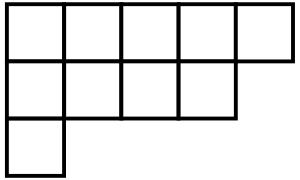
\includegraphics[width = 3cm]{fig1.png}
		\end{center}
		
		Chamaremos de partição \emph{conjugada} a partição que obtemos ao refletir o Young tableau. Por exemplo, a partição conjugada de $(5, 4, 1)$ é $(3, 2, 2, 2, 1)$, representada por:
		\begin{center}
			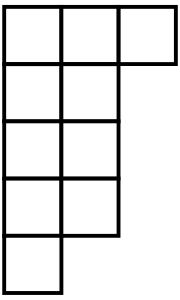
\includegraphics[height = 3cm]{fig2.png}
		\end{center}

		Desse modo, podemos ver que há uma bijeção entre o conjunto de partições de $n$ com maior parte exatamente $r$ e o conjunto de partições de $n$ em $r$ partes, definida por essa conjugação.
	\end{sol}


	%\begin{prob}
	%	Prove que o número de partições de $n$ em que apenas as partes ímpares podem ser repetidas é igual ao número de partições de $n$ em que nenhum parte aparece mais do que $3$ vezes.
	%\end{prob}

	\newpage
	\setcounter{prob}{3}

	\begin{prob}
		Prove que o número de partições de $n$ em partes distintas é igual ao número de partições de $n$ em partes ímpares.
	\end{prob}

	\begin{sol}[Funções geratrizes]
		Seja $f(x)$ a função geratriz que gera o número de partições de $n$ em partes distintas.
		Seja $g(x)$ a função geratriz que gera o número de partições de $n$ em partes ímpares.

		\begin{align*}
			f(x) & = \prod_{i=1}^{\infty} (1+x^i)\\
				 & = \frac{\prod_{i=1}^{\infty} (1-x^{2i})}{\prod_{i=1}^{\infty} (1-x^i)}\\ 
				 & = \frac{\prod_{i\text{ par}} (1-x^i)}{\prod_{i=1}^{\infty} (1-x^i)}\\
				 & = \prod_{i\text{ ímpar}} \frac{1}{1-x^i} \\
			g(x) & = \prod_{k\text{ ímpar}} (1 + x^k + (x^k)^2 + (x^k)^3 + \cdots)\\
				 & = \prod_{k\text{ ímpar}} \frac{1}{1-x^k},\\
		\end{align*}
		que prova que $f(x) = g(x)$.

		Outro jeito é mostrar que $\frac{f(x)}{g(x)} = 1$, que indica um pouco mais da relação entre essa solução e a solução usando bijeções:
		\begin{lem}
			\[\prod_{\alpha = 0}^{\infty} (1+x^{2^\alpha}) = \sum_{t=0}^{\infty} x^t = \frac{1}{1-x}\]
		\end{lem}

		\begin{align*}
			\frac{f(x)}{g(x)} & = \prod_{i=1}^{\infty} (1+x^i) \cdot \prod_{k\text{ ímpar}} (1-x^k)\\
							  & = \prod_{k\text{ ímpar}} \prod_{\alpha = 0}^{\infty} (1+x^{k2^\alpha}) \cdot \prod_{k\text{ ímpar}} (1-x^k)\\
							  & = \prod_{k\text{ ímpar}} \left(\prod_{\alpha = 0}^{\infty} (1+(x^k)^{2^\alpha})\right) (1-x^k)\\
						  	  & = 1
		\end{align*}

	\end{sol}

	%\begin{prob}
	%	O conjunto $A$ é um subconjunto de $\{1, 2, 3, \dots, n\}$ tal que $A+A = \{a+b : a, b \in A\}$ não intersecta $A$. Ache, em função de $n$, o número máximo de elementos de $A$.
	%\end{prob}

	\newpage

	\section{Questões Divertidas}

	%\begin{prob}
	%	Seja $n$ um inteiro positivo. Alice e Bruno jogam o seguinte jogo: eles constroem uma partição de $n$ da seguinte forma: Inicialmente, Alice escolhe um inteiro positivo $a_1 < n$. Depois Bruno escolhe um inteiro positivo $a_2 \le a_1$ tal que $a_1 + a_2 \le n$. Em seguida, Alice escolhe um inteiro positivo $a_3 \le a_2$ tal que $a_1 + a_2 + a_3 \le n$. O jogo continua, alternando os jogadores, até obtermos uma partição $a_1 + a_2 + \cdots + a_k$ de $n$. Se $k$ é ímpar, Alice vence; caso contrário, Bruno vence. Determine, em função de $n$, quem tem a estratégia vencedora.
	%\end{prob}

	\setcounter{prob}{1}

	\problem{math/imo/1997/6}

	\noindent \textit{Rascunho.} Quanto é $f(2k+1)$?
	\[ f(2k+1) = f(2k).\]

	Quanto é $f(2k)$, exatamente?
	\[f(2k) = f(k) + f(2(k-1))\]
	
	Somando a expressão acima, temos
	\begin{align*}
		\sum_{k=1}^{n} f(2k) & = \sum_{k=1}^{n} f(k) + \sum_{k=1}^{n} f(2(k-1))\\
		f(2n) & = \sum_{k=1}^{n} f(k) + f(0)\\
		f(2n) & = \sum_{k=0}^{n} f(k)
	\end{align*}

	Provando a desigualdade superior, temos:

	\begin{align*}
		f(2^n) & = \sum_{k=0}^{2^{n-1}} f(k) \\
			   & \le (2^{n-1})f(2^{n-1}) + 1\\
			   & < (2^{n-1})2^{\frac{(n-1)^2}{2}}\\
			   & < 2^\frac{n^2}{2}
	\end{align*}

	Tentando provar a desigualdade superior, temos:

	\begin{align*}
		f(2^n) & = \sum_{k=0}^{2^{n-1}} f(k) \\
			   & = \left(\sum_{k=2^{n-2}+1}^{2^{n-1}} f(k)\right) + \left(\sum_{k=0}^{2^{n-2}} f(k)\right) \\
			   & = \left(\sum_{k=2^{n-2}+1}^{2^{n-1}} f(k)\right) + f(2^{n-1}) \\
			   & \ge 2^{n-2}f(2^{n-2}) + f(2^{n-1})\\
			   & > 2^{n-2}2^\frac{n^2-4n+4}{4} + 2^\frac{n^2-2n+1}{4}\\
			   & > 2^\frac{n^2 - 4}{4} + 2^\frac{n^2 - 2n + 2}{4},
	\end{align*}
	que não dá a cota certa.

	%\begin{align*}
	%	f(2^n) & = 2 \cdot \sum_{i=0}^{2^{n-2}} f(2^{n-1}-2i) \\
	%		   & = 2 \cdot \sum_{i=0}^{2^{n-2}-1} f(2^{n-1}-2i) + 2\\
	%		   & = 2 \cdot \left(\sum_{i=0}^{2^{n-2}-1} f(2^{n-2}-i) + \sum_{i=0}^{2^{n-2}-1} f(2 \cdot(2^{n-2}-i - 1))\right) + 2\\
	%		   & = 2 \cdot \left(\sum_{i=0}^{2^{n-2}} f(2^{n-2}-i) + \sum_{i=0}^{2^{n-2}-1} f(2 \cdot(2^{n-2}-i-1))\right)\\
	%		   & = 2 \cdot \left(f(2^{n-2}) + \sum_{i=0}^{2^{n-2}-1} f(2 \cdot(2^{n-2}-i-1))\right)
	%\end{align*}

	%\problem{math/imo/1992/6}

	%\begin{prob}[Yufei Zhao \cite{Combinatorics3-YZhao}]
	%	Determine se existe um subconjunto $S$ dos inteiros positivos com a seguinte propriedade: para todo inteiro positivo $n$, o número de partições de $n$, onde cada parte aparece no máximo duas vezes, é igual ao número de partições de $n$ em partes que são elementos de $S$.
	%\end{prob}

	%\newpage
	%\section{Problemas Interessantes}

	%\problem{math/miklos_schweitzer/2009/3}

	%\setcounter{prob}{1}

	%\problem{math/imosl/2015/C6}
	
	%\problem{math/apmo/2020/3}


	%\begin{prob}
	%	Definimos o \emph{espectro} de um número real $\alpha$ como a sequência \[\Spec(\alpha) = (\floor{\alpha}, \floor{2\alpha}, \floor{3\alpha}, \dots).\]
	%	\begin{enumerate}[label = (\alph*)]
	%		\item \textbf{(Beatty's Theorem, 1926)} Se $\alpha > 1$ é um irracional e $\frac{1}{\alpha} + \frac{1}{\beta} = 1$, mostre que as sequências $\Spec(\alpha)$ e $\Spec(\beta)$ particionam os inteiros positivos. Em outras palavras, mostre que $\Spec(\alpha) \cup \Spec(\beta) = \ZZ_{>0}$ e $\Spec(\alpha) \cap \Spec(\beta) = \varnothing$. 
	%		\item \textbf{(Bang’s Theorem, 1957)} Prove a recíproca do teorema acima.
	%	\end{enumerate}
	%\end{prob}

	%\section{Desafio Final}

	%\problem{math/imosl/2010/C7}

	\newpage

	\bibliographystyle{plain}
	%\bibliography{mybib}{}

	\bibliography{mybib}
	%\printbibliography
\end{document}
